% Generated 2020-01-09 18:51:19 -0800
\subsection{Data Items} \label{model:DataItems}

\begin{figure}[ht]
  \centering
    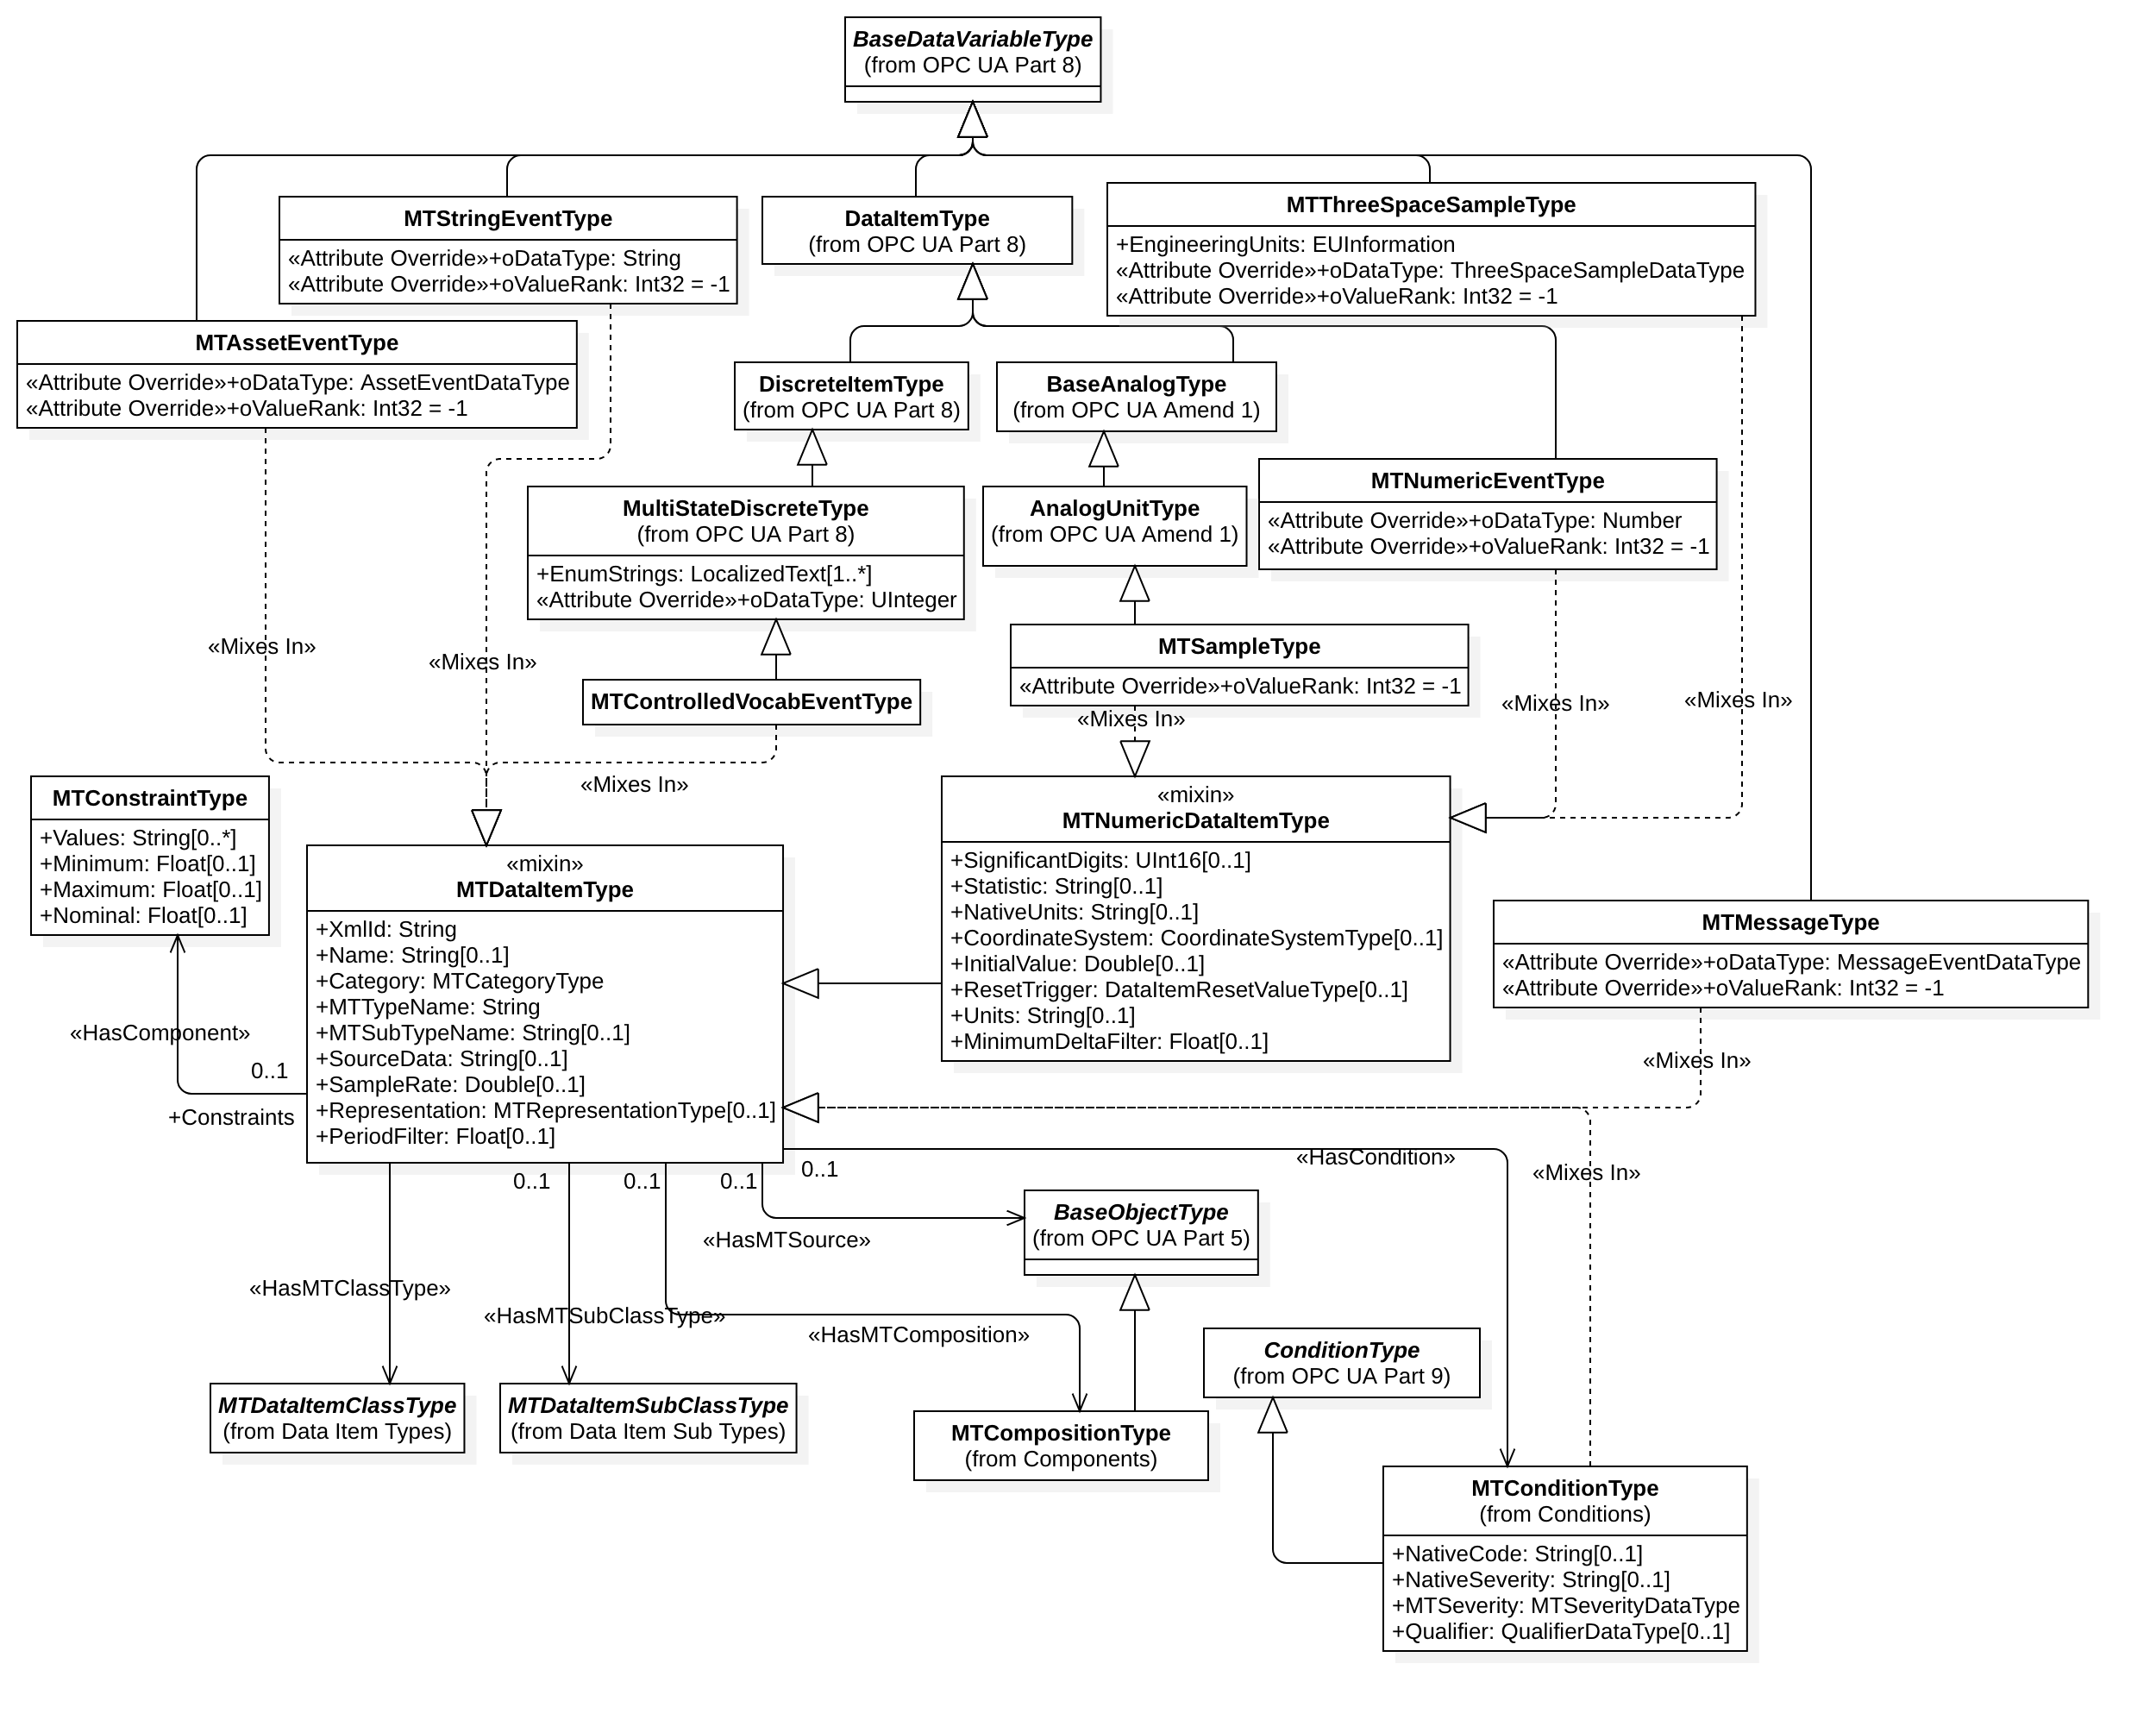
\includegraphics[width=1.0\textwidth]{./diagrams/types/DataItems.png}
  \caption{Data Items Diagram}
  \label{fig:DataItems}
\end{figure}

\FloatBarrier


\input ./type-sections/DataItems.tex

\subsubsection{Defintion of \texttt{ AssetEventDataType}}
  \label{type:AssetEventDataType}

\FloatBarrier

A special \gls{Variable} data type for asset change with a \mtmodel{AssetType} and \mtmodel{AssetId}.

\begin{table}[ht]
\centering 
  \caption{\texttt{AssetEventDataType} DataType}
  \label{data-type:AssetEventDataType}
\tabulinesep=3pt
\begin{tabu} to 6in {|l|l|l|} \everyrow{\hline}
\hline
\rowfont\bfseries {Field} & {Type} & {Optional} \\
\tabucline[1.5pt]{}
\texttt{AssetId} & \texttt{String} & \texttt{Mandatory} \\
\texttt{AssetType} & \texttt{String} & \texttt{Mandatory} \\
\end{tabu}
\end{table} 

\FloatBarrier
\subsubsection{Defintion of \texttt{ MTAssetEventType}}
  \label{type:MTAssetEventType}

\FloatBarrier

The asset events have an additional attribute regarding the asset change or removal identifier
and the type of asset that is being reported.

\begin{table}[ht]
\centering 
  \caption{\texttt{MTAssetEventType} Definition}
  \label{table:MTAssetEventType}
\fontsize{9pt}{11pt}\selectfont
\tabulinesep=3pt
\begin{tabu} to 6in {|X[-1.35]|X[-0.7]|X[-1.75]|X[-1.5]|X[-1]|X[-0.7]|} \everyrow{\hline}
\hline
\rowfont\bfseries {Attribute} & \multicolumn{5}{|l|}{Value} \\
\tabucline[1.5pt]{}
BrowseName & \multicolumn{5}{|l|}{MTAssetEventType} \\
IsAbstract & \multicolumn{5}{|l|}{False} \\
ValueRank & \multicolumn{5}{|l|}{-1} \\
DataType & \multicolumn{5}{|l|}{AssetEventDataType} \\
\tabucline[1.5pt]{}
\rowfont \bfseries References & NodeClass & BrowseName & DataType & Type\-Definition & {Modeling\-Rule} \\
\multicolumn{6}{|l|}{Subtype of BaseDataVariableType (See \cite{UAPart8} Documentation)} \\
Has\-Property & Variable & Category & MT\-Category\-Type & Property\-Type & Mandatory \\
Has\-Property & Variable & MT\-Sub\-Type\-Name & String & Property\-Type & Optional \\
Has\-Property & Variable & MT\-Type\-Name & String & Property\-Type & Mandatory \\
Has\-Property & Variable & Name & String & Property\-Type & Optional \\
Has\-Property & Variable & Period\-Filter & Float & Property\-Type & Optional \\
Has\-Property & Variable & Representation & MT\-Representation\-Type & Property\-Type & Optional \\
Has\-Property & Variable & Sample\-Rate & Double & Property\-Type & Optional \\
Has\-Property & Variable & Source\-Data & String & Property\-Type & Optional \\
Has\-Property & Variable & Xml\-Id & String & Property\-Type & Mandatory \\
Has\-MT\-Source & Object & <Base\-Object> & \multicolumn{2}{l|}{BaseObjectType} & Optional \\
Has\-MT\-Composition & Object & <MT\-Composition> & \multicolumn{2}{l|}{MTCompositionType} & Optional \\
Has\-MT\-Sub\-Class\-Type & Object & <MT\-Data\-Item\-Sub\-Class> & \multicolumn{2}{l|}{MTDataItemSubClassType} & Optional \\
Has\-Condition & Object & <MT\-Condition> & \multicolumn{2}{l|}{MTConditionType} & Optional \\
Has\-Component & Object & Constraints & \multicolumn{2}{l|}{MTConstraintType} & Optional \\
Has\-MT\-Class\-Type & Object & <MT\-Data\-Item\-Class> & \multicolumn{2}{l|}{MTDataItemClassType} & Mandatory \\
\end{tabu}
\end{table} 


\paragraph{Dependencies and Relationships}

\begin{itemize}
\item Mixes in \texttt{MTDataItemType}, see See section \ref{type:MTDataItemType}
\end{itemize}
\FloatBarrier
\subsubsection{Defintion of \texttt{ MTConditionClassType}}
  \label{type:MTConditionClassType}

\FloatBarrier

The abstract type for all data items types that are specifically for \mtmodel{CONDITION} \gls{category}.

An XML element which provides the information and data reported from a piece of equipment for those dataitem elements defined with a category attribute of condition category in the mtconnectdevices document.

\begin{table}[ht]
\centering 
  \caption{\texttt{MTConditionClassType} Definition}
  \label{table:MTConditionClassType}
\fontsize{9pt}{11pt}\selectfont
\tabulinesep=3pt
\begin{tabu} to 6in {|X[-1.35]|X[-0.7]|X[-1.75]|X[-1.5]|X[-1]|X[-0.7]|} \everyrow{\hline}
\hline
\rowfont\bfseries {Attribute} & \multicolumn{5}{|l|}{Value} \\
\tabucline[1.5pt]{}
BrowseName & \multicolumn{5}{|l|}{MTConditionClassType} \\
IsAbstract & \multicolumn{5}{|l|}{True} \\
\tabucline[1.5pt]{}
\rowfont \bfseries References & NodeClass & BrowseName & DataType & Type\-Definition & {Modeling\-Rule} \\
\multicolumn{6}{|l|}{Subtype of MTDataItemClassType (See Data Item Types Documentation)} \\
HasSubtype & ObjectType & \multicolumn{2}{l}{ActuatorClassType} & \multicolumn{2}{|l|}{See section \ref{type:ActuatorClassType}} \\
HasSubtype & ObjectType & \multicolumn{2}{l}{CommunicationsClassType} & \multicolumn{2}{|l|}{See section \ref{type:CommunicationsClassType}} \\
HasSubtype & ObjectType & \multicolumn{2}{l}{DataRangeClassType} & \multicolumn{2}{|l|}{See section \ref{type:DataRangeClassType}} \\
HasSubtype & ObjectType & \multicolumn{2}{l}{HardwareClassType} & \multicolumn{2}{|l|}{See section \ref{type:HardwareClassType}} \\
HasSubtype & ObjectType & \multicolumn{2}{l}{LogicProgramClassType} & \multicolumn{2}{|l|}{See section \ref{type:LogicProgramClassType}} \\
HasSubtype & ObjectType & \multicolumn{2}{l}{MotionProgramClassType} & \multicolumn{2}{|l|}{See section \ref{type:MotionProgramClassType}} \\
HasSubtype & ObjectType & \multicolumn{2}{l}{SystemClassType} & \multicolumn{2}{|l|}{See section \ref{type:SystemClassType}} \\
\end{tabu}
\end{table} 


\FloatBarrier
\subsubsection{Defintion of \texttt{ MTConstraintType}}
  \label{type:MTConstraintType}

\FloatBarrier

The MTConnect constraints. The Values or the Minimum, Maximum, and Nominal values should be 
provided. Multiple Values can be provided as an array as a set of allowable values for this
\gls{MTDataItem}.

A constraint is used by a software application to evaluate the validity of the reported data.

\begin{table}[ht]
\centering 
  \caption{\texttt{MTConstraintType} Definition}
  \label{table:MTConstraintType}
\fontsize{9pt}{11pt}\selectfont
\tabulinesep=3pt
\begin{tabu} to 6in {|X[-1.35]|X[-0.7]|X[-1.75]|X[-1.5]|X[-1]|X[-0.7]|} \everyrow{\hline}
\hline
\rowfont\bfseries {Attribute} & \multicolumn{5}{|l|}{Value} \\
\tabucline[1.5pt]{}
BrowseName & \multicolumn{5}{|l|}{MTConstraintType} \\
IsAbstract & \multicolumn{5}{|l|}{False} \\
\tabucline[1.5pt]{}
\rowfont \bfseries References & NodeClass & BrowseName & DataType & Type\-Definition & {Modeling\-Rule} \\
\multicolumn{6}{|l|}{Subtype of BaseObjectType (See \cite{UAPart5} Documentation)} \\
Has\-Property & Variable & Maximum & Float & Property\-Type & Optional \\
Has\-Property & Variable & Minimum & Float & Property\-Type & Optional \\
Has\-Property & Variable & Nominal & Float & Property\-Type & Optional \\
Has\-Property & Variable & Values & String[] & Property\-Type & Optional \\
\end{tabu}
\end{table} 


\FloatBarrier
\subsubsection{Defintion of \texttt{ MTControlledVocabEventType}}
  \label{type:MTControlledVocabEventType}

\FloatBarrier

All \glspl{MTDataItem} with \gls{category} \mtmodel{EVENT} having Controlled Vocabularies (Enumerations) 
will be added as sub-types of this type which is mapped to the OPC/UA MultiStateValueDiscreteType. 
Otherwise, either \mtmodel{MTString} or \mtmodel{MTNumeric} will be used. All subtypes are direct representations of the 
MTConnect equivalent elements that can be found in the MTConnect Part 3 \cite{MTCPart3} documents.

\begin{table}[ht]
\centering 
  \caption{\texttt{MTControlledVocabEventType} Definition}
  \label{table:MTControlledVocabEventType}
\fontsize{9pt}{11pt}\selectfont
\tabulinesep=3pt
\begin{tabu} to 6in {|X[-1.35]|X[-0.7]|X[-1.75]|X[-1.5]|X[-1]|X[-0.7]|} \everyrow{\hline}
\hline
\rowfont\bfseries {Attribute} & \multicolumn{5}{|l|}{Value} \\
\tabucline[1.5pt]{}
BrowseName & \multicolumn{5}{|l|}{MTControlledVocabEventType} \\
IsAbstract & \multicolumn{5}{|l|}{False} \\
ValueRank & \multicolumn{5}{|l|}{-1} \\
DataType & \multicolumn{5}{|l|}{UInteger} \\
\tabucline[1.5pt]{}
\rowfont \bfseries References & NodeClass & BrowseName & DataType & Type\-Definition & {Modeling\-Rule} \\
\multicolumn{6}{|l|}{Subtype of MultiStateDiscreteType (See \cite{UAPart8} Documentation)} \\
Has\-Property & Variable & Category & MT\-Category\-Type & Property\-Type & Mandatory \\
Has\-Property & Variable & MT\-Sub\-Type\-Name & String & Property\-Type & Optional \\
Has\-Property & Variable & MT\-Type\-Name & String & Property\-Type & Mandatory \\
Has\-Property & Variable & Name & String & Property\-Type & Optional \\
Has\-Property & Variable & Period\-Filter & Float & Property\-Type & Optional \\
Has\-Property & Variable & Representation & MT\-Representation\-Type & Property\-Type & Optional \\
Has\-Property & Variable & Sample\-Rate & Double & Property\-Type & Optional \\
Has\-Property & Variable & Source\-Data & String & Property\-Type & Optional \\
Has\-Property & Variable & Xml\-Id & String & Property\-Type & Mandatory \\
Has\-MT\-Source & Object & <Base\-Object> & \multicolumn{2}{l|}{BaseObjectType} & Optional \\
Has\-MT\-Composition & Object & <MT\-Composition> & \multicolumn{2}{l|}{MTCompositionType} & Optional \\
Has\-MT\-Sub\-Class\-Type & Object & <MT\-Data\-Item\-Sub\-Class> & \multicolumn{2}{l|}{MTDataItemSubClassType} & Optional \\
Has\-Condition & Object & <MT\-Condition> & \multicolumn{2}{l|}{MTConditionType} & Optional \\
Has\-Component & Object & Constraints & \multicolumn{2}{l|}{MTConstraintType} & Optional \\
Has\-MT\-Class\-Type & Object & <MT\-Data\-Item\-Class> & \multicolumn{2}{l|}{MTDataItemClassType} & Mandatory \\
Has\-Property & Variable & Value\-As\-Text & String & Property\-Type & Mandatory \\
\end{tabu}
\end{table} 


\paragraph{Dependencies and Relationships}

\begin{itemize}
\item Mixes in \texttt{MTDataItemType}, see See section \ref{type:MTDataItemType}
\end{itemize}
\FloatBarrier
\subsubsection{Defintion of \texttt{<<mixin>> MTDataItemType}}
  \label{type:MTDataItemType}

\FloatBarrier

The data item mixin will inject the properties and the methods into the related 
classes. This facility is similar to the Ruby module mixin or the Scala traits.

data entity describing a piece of information reported about a piece of equipment.

\begin{table}[ht]
\centering 
  \caption{\texttt{MTDataItemType} Definition}
  \label{table:MTDataItemType}
\fontsize{9pt}{11pt}\selectfont
\tabulinesep=3pt
\begin{tabu} to 6in {|X[-1.35]|X[-0.7]|X[-1.75]|X[-1.5]|X[-1]|X[-0.7]|} \everyrow{\hline}
\hline
\rowfont\bfseries {Attribute} & \multicolumn{5}{|l|}{Value} \\
\tabucline[1.5pt]{}
BrowseName & \multicolumn{5}{|l|}{MTDataItemType} \\
IsAbstract & \multicolumn{5}{|l|}{False} \\
\tabucline[1.5pt]{}
\rowfont \bfseries References & NodeClass & BrowseName & DataType & Type\-Definition & {Modeling\-Rule} \\
HasSubtype & ObjectType & \multicolumn{2}{l}{MTNumericDataItemType} & \multicolumn{2}{|l|}{See section \ref{type:MTNumericDataItemType}} \\
Has\-Property & Variable & Category & MT\-Category\-Type & Property\-Type & Mandatory \\
Has\-Property & Variable & MT\-Sub\-Type\-Name & String & Property\-Type & Optional \\
Has\-Property & Variable & MT\-Type\-Name & String & Property\-Type & Mandatory \\
Has\-Property & Variable & Name & String & Property\-Type & Optional \\
Has\-Property & Variable & Period\-Filter & Float & Property\-Type & Optional \\
Has\-Property & Variable & Representation & MT\-Representation\-Type & Property\-Type & Optional \\
Has\-Property & Variable & Sample\-Rate & Double & Property\-Type & Optional \\
Has\-Property & Variable & Source\-Data & String & Property\-Type & Optional \\
Has\-Property & Variable & Xml\-Id & String & Property\-Type & Mandatory \\
Has\-MT\-Source & Object & <Base\-Object> & \multicolumn{2}{l|}{BaseObjectType} & Optional \\
Has\-MT\-Composition & Object & <MT\-Composition> & \multicolumn{2}{l|}{MTCompositionType} & Optional \\
Has\-MT\-Sub\-Class\-Type & Object & <MT\-Data\-Item\-Sub\-Class> & \multicolumn{2}{l|}{MTDataItemSubClassType} & Optional \\
Has\-Condition & Object & <MT\-Condition> & \multicolumn{2}{l|}{MTConditionType} & Optional \\
Has\-Component & Object & Constraints & \multicolumn{2}{l|}{MTConstraintType} & Optional \\
Has\-MT\-Class\-Type & Object & <MT\-Data\-Item\-Class> & \multicolumn{2}{l|}{MTDataItemClassType} & Mandatory \\
\end{tabu}
\end{table} 


\FloatBarrier
\paragraph{Referenced Properties and Objects}

\begin{itemize}
\item \textbf{Allowable Values} for \texttt{MTCategoryType}
\FloatBarrier

Represents the \gls{category} attribute of the MTConnect \gls{MTDataItem}.

\begin{table}[ht]
\centering 
  \caption{\texttt{MTCategoryType} Enumeration}
  \label{enum:MTCategoryType}
\tabulinesep=3pt
\begin{tabu} to 6in {|l|r|} \everyrow{\hline}
\hline
\rowfont\bfseries {Name} & {Index} \\
\tabucline[1.5pt]{}
\texttt{EVENT} & \texttt{0} \\
\texttt{CONDITION} & \texttt{1} \\
\texttt{SAMPLE} & \texttt{2} \\
\end{tabu}
\end{table} 
\FloatBarrier
\item \texttt{PeriodFilter::Float:} Represents the MTConnect \mtmodel{Filter} subtype of \mtmodel{PeriodFilter}.

\item \textbf{Allowable Values} for \texttt{MTRepresentationType}
\FloatBarrier

Represents the \mtmodel{representation} attribute of the MTConnect \gls{MTDataItem}.

\begin{table}[ht]
\centering 
  \caption{\texttt{MTRepresentationType} Enumeration}
  \label{enum:MTRepresentationType}
\tabulinesep=3pt
\begin{tabu} to 6in {|l|r|} \everyrow{\hline}
\hline
\rowfont\bfseries {Name} & {Index} \\
\tabucline[1.5pt]{}
\texttt{DISCRETE} & \texttt{0} \\
\texttt{TIME_SERIES} & \texttt{1} \\
\texttt{VALUE} & \texttt{2} \\
\end{tabu}
\end{table} 
\FloatBarrier
\item \texttt{SourceData::String:} The text that is the \gls{CDATA} of the \mtmodel{Source} element.

\end{itemize}
\FloatBarrier
\subsubsection{Defintion of \texttt{<<mixin>> MTNumericDataItemType}}
  \label{type:MTNumericDataItemType}

\FloatBarrier

These are the additional attributes that are relevent to numeric data items. 
The factory will evaluate these values and will set the engineering units and the 
range associated with the parent entity.

\begin{table}[ht]
\centering 
  \caption{\texttt{MTNumericDataItemType} Definition}
  \label{table:MTNumericDataItemType}
\fontsize{9pt}{11pt}\selectfont
\tabulinesep=3pt
\begin{tabu} to 6in {|X[-1.35]|X[-0.7]|X[-1.75]|X[-1.5]|X[-1]|X[-0.7]|} \everyrow{\hline}
\hline
\rowfont\bfseries {Attribute} & \multicolumn{5}{|l|}{Value} \\
\tabucline[1.5pt]{}
BrowseName & \multicolumn{5}{|l|}{MTNumericDataItemType} \\
IsAbstract & \multicolumn{5}{|l|}{False} \\
\tabucline[1.5pt]{}
\rowfont \bfseries References & NodeClass & BrowseName & DataType & Type\-Definition & {Modeling\-Rule} \\
\multicolumn{6}{|l|}{Subtype of MTDataItemType (See section \ref{type:MTDataItemType})} \\
Has\-Property & Variable & Coordinate\-System & MT\-Coordinate\-System\-Type & Property\-Type & Optional \\
Has\-Property & Variable & Duration & Duration & Property\-Type & Optional \\
Has\-Property & Variable & Initial\-Value & Double & Property\-Type & Optional \\
Has\-Property & Variable & Minimum\-Delta\-Filter & Float & Property\-Type & Optional \\
Has\-Property & Variable & Native\-Units & String & Property\-Type & Optional \\
Has\-Property & Variable & Reset\-Trigger & MT\-Reset\-Trigger\-Type & Property\-Type & Optional \\
Has\-Property & Variable & Reset\-Triggered\-Reason & MT\-Reset\-Trigger\-Type & Property\-Type & Optional \\
Has\-Property & Variable & Significant\-Digits & Int16 & Property\-Type & Optional \\
Has\-Property & Variable & Statistic & MT\-Statistic\-Type & Property\-Type & Optional \\
Has\-Property & Variable & Units & String & Property\-Type & Optional \\
\end{tabu}
\end{table} 


\FloatBarrier
\paragraph{Referenced Properties and Objects}

\begin{itemize}
\item \textbf{Allowable Values} for \texttt{MTCoordinateSystemType}
\FloatBarrier

Represents the \mtmodel{coordinateSystem} attribute of the MTConnect \gls{MTDataItem}.

\begin{table}[ht]
\centering 
  \caption{\texttt{MTCoordinateSystemType} Enumeration}
  \label{enum:MTCoordinateSystemType}
\tabulinesep=3pt
\begin{tabu} to 6in {|l|r|} \everyrow{\hline}
\hline
\rowfont\bfseries {Name} & {Index} \\
\tabucline[1.5pt]{}
\texttt{MACHINE} & \texttt{0} \\
\texttt{WORK} & \texttt{1} \\
\end{tabu}
\end{table} 
\FloatBarrier
\item \texttt{MinimumDeltaFilter::Float:} Represents the MTConnect \mtmodel{Filter} subtype of \mtmodel{MinimumDeltaFilter}.

\item \texttt{ResetTrigger::MTResetTriggerType:} If a \mtmodel{ResetTrigger} is given, when an \mtmodel{resetTriggered} attribtue is given in an event, the \uamodel{StatusCode} MUST have bit 14 set \uamodel{SemanticsChanged} and the \mtmodel{ResetTriggeredReason} must be set to the value of the \mtmodel{resetTriggered} attribute.

\item \textbf{Allowable Values} for \texttt{MTResetTriggerType}
\FloatBarrier

These need to become \uamodel{Good_} status code in OPC UA.

resettrigger is an optional XML element that identifies the type of event that may cause a reset to occur. It is additional information regarding the meaning of the data that establishes an understanding of the time frame that the data represents so that the data may be correctly understood by a client software application.

\begin{table}[ht]
\centering 
  \caption{\texttt{MTResetTriggerType} Enumeration}
  \label{enum:MTResetTriggerType}
\tabulinesep=3pt
\begin{tabu} to 6in {|l|r|} \everyrow{\hline}
\hline
\rowfont\bfseries {Name} & {Index} \\
\tabucline[1.5pt]{}
\texttt{ACTION_COMPLETE} & \texttt{0} \\
\texttt{ANNUAL} & \texttt{1} \\
\texttt{DAY} & \texttt{2} \\
\texttt{MAINTENANCE} & \texttt{3} \\
\texttt{MANUAL} & \texttt{4} \\
\texttt{MONTH} & \texttt{5} \\
\texttt{POWER_ON} & \texttt{6} \\
\texttt{SHIFT} & \texttt{7} \\
\texttt{WEEK} & \texttt{8} \\
\end{tabu}
\end{table} 
\FloatBarrier
\item \textbf{Allowable Values} for \texttt{MTResetTriggerType}
\FloatBarrier

These need to become \uamodel{Good_} status code in OPC UA.

resettrigger is an optional XML element that identifies the type of event that may cause a reset to occur. It is additional information regarding the meaning of the data that establishes an understanding of the time frame that the data represents so that the data may be correctly understood by a client software application.

\begin{table}[ht]
\centering 
  \caption{\texttt{MTResetTriggerType} Enumeration}
\tabulinesep=3pt
\begin{tabu} to 6in {|l|r|} \everyrow{\hline}
\hline
\rowfont\bfseries {Name} & {Index} \\
\tabucline[1.5pt]{}
\texttt{ACTION_COMPLETE} & \texttt{0} \\
\texttt{ANNUAL} & \texttt{1} \\
\texttt{DAY} & \texttt{2} \\
\texttt{MAINTENANCE} & \texttt{3} \\
\texttt{MANUAL} & \texttt{4} \\
\texttt{MONTH} & \texttt{5} \\
\texttt{POWER_ON} & \texttt{6} \\
\texttt{SHIFT} & \texttt{7} \\
\texttt{WEEK} & \texttt{8} \\
\end{tabu}
\end{table} 
\FloatBarrier
\item \texttt{SignificantDigits::Int16:} The significant digits is converted to a \uaterm{ValuePrecision}.

\item \textbf{Allowable Values} for \texttt{MTStatisticType}
\FloatBarrier



\begin{table}[ht]
\centering 
  \caption{\texttt{MTStatisticType} Enumeration}
  \label{enum:MTStatisticType}
\tabulinesep=3pt
\begin{tabu} to 6in {|l|r|} \everyrow{\hline}
\hline
\rowfont\bfseries {Name} & {Index} \\
\tabucline[1.5pt]{}
\texttt{AVERAGE} & \texttt{0} \\
\texttt{MAXIMUM} & \texttt{1} \\
\texttt{MEDIAN} & \texttt{2} \\
\texttt{MINIMUM} & \texttt{3} \\
\texttt{MODE} & \texttt{4} \\
\texttt{RANGE} & \texttt{5} \\
\texttt{ROOT_MEAN_SQUARE} & \texttt{6} \\
\texttt{STANDARD_DEVIATION} & \texttt{7} \\
\end{tabu}
\end{table} 
\FloatBarrier
\end{itemize}
\FloatBarrier
\subsubsection{Defintion of \texttt{ MTEventClassType}}
  \label{type:MTEventClassType}

\FloatBarrier

The base type class for all data items with a \gls{category} of \mtmodel{EVENT}.

An XML element which provides the information and data reported from a piece of equipment for those dataitem elements defined with a category attribute of event category in the mtconnectdevices document.

\begin{table}[ht]
\centering 
  \caption{\texttt{MTEventClassType} Definition}
  \label{table:MTEventClassType}
\fontsize{9pt}{11pt}\selectfont
\tabulinesep=3pt
\begin{tabu} to 6in {|X[-1.35]|X[-0.7]|X[-1.75]|X[-1.5]|X[-1]|X[-0.7]|} \everyrow{\hline}
\hline
\rowfont\bfseries {Attribute} & \multicolumn{5}{|l|}{Value} \\
\tabucline[1.5pt]{}
BrowseName & \multicolumn{5}{|l|}{MTEventClassType} \\
IsAbstract & \multicolumn{5}{|l|}{True} \\
\tabucline[1.5pt]{}
\rowfont \bfseries References & NodeClass & BrowseName & DataType & Type\-Definition & {Modeling\-Rule} \\
\multicolumn{6}{|l|}{Subtype of MTDataItemClassType (See Data Item Types Documentation)} \\
HasSubtype & ObjectType & \multicolumn{2}{l}{MTMessageClassType} & \multicolumn{2}{|l|}{See section \ref{type:MTMessageClassType}} \\
HasSubtype & ObjectType & \multicolumn{2}{l}{MTControlledVocabEventClassType} & \multicolumn{2}{|l|}{See section \ref{type:MTControlledVocabEventClassType}} \\
HasSubtype & ObjectType & \multicolumn{2}{l}{MTNumericEventClassType} & \multicolumn{2}{|l|}{See section \ref{type:MTNumericEventClassType}} \\
HasSubtype & ObjectType & \multicolumn{2}{l}{MTStringEventClassType} & \multicolumn{2}{|l|}{See section \ref{type:MTStringEventClassType}} \\
\end{tabu}
\end{table} 


\FloatBarrier
\subsubsection{Defintion of \texttt{ MTMessageEventType}}
  \label{type:MTMessageEventType}

\FloatBarrier



\begin{table}[ht]
\centering 
  \caption{\texttt{MTMessageEventType} Definition}
  \label{table:MTMessageEventType}
\fontsize{9pt}{11pt}\selectfont
\tabulinesep=3pt
\begin{tabu} to 6in {|X[-1.35]|X[-0.7]|X[-1.75]|X[-1.5]|X[-1]|X[-0.7]|} \everyrow{\hline}
\hline
\rowfont\bfseries {Attribute} & \multicolumn{5}{|l|}{Value} \\
\tabucline[1.5pt]{}
BrowseName & \multicolumn{5}{|l|}{MTMessageEventType} \\
IsAbstract & \multicolumn{5}{|l|}{False} \\
\tabucline[1.5pt]{}
\rowfont \bfseries References & NodeClass & BrowseName & DataType & Type\-Definition & {Modeling\-Rule} \\
\multicolumn{6}{|l|}{Subtype of BaseEventType (See \cite{UAPart5} Documentation)} \\
Has\-Property & Variable & Native\-Code & String & Property\-Type & Optional \\
\end{tabu}
\end{table} 


\FloatBarrier
\subsubsection{Defintion of \texttt{ MTMessageType}}
  \label{type:MTMessageType}

\FloatBarrier

The message is a sub-type of the \uaterm{DataVariableType} using the \mtuatype{MessageDataType} to 
represent the values for \mtterm{NativeCode} and \mtterm{Text} of the message from the \gls{CDATA} of the 
MTConnect Streams message.

Any text string of information to be transferred from a piece of equipment to a client software application.

\begin{table}[ht]
\centering 
  \caption{\texttt{MTMessageType} Definition}
  \label{table:MTMessageType}
\fontsize{9pt}{11pt}\selectfont
\tabulinesep=3pt
\begin{tabu} to 6in {|X[-1.35]|X[-0.7]|X[-1.75]|X[-1.5]|X[-1]|X[-0.7]|} \everyrow{\hline}
\hline
\rowfont\bfseries {Attribute} & \multicolumn{5}{|l|}{Value} \\
\tabucline[1.5pt]{}
BrowseName & \multicolumn{5}{|l|}{MTMessageType} \\
IsAbstract & \multicolumn{5}{|l|}{False} \\
ValueRank & \multicolumn{5}{|l|}{-1} \\
DataType & \multicolumn{5}{|l|}{MessageDataType} \\
\tabucline[1.5pt]{}
\rowfont \bfseries References & NodeClass & BrowseName & DataType & Type\-Definition & {Modeling\-Rule} \\
\multicolumn{6}{|l|}{Subtype of BaseDataVariableType (See \cite{UAPart8} Documentation)} \\
Has\-Property & Variable & Category & MT\-Category\-Type & Property\-Type & Mandatory \\
Has\-Property & Variable & MT\-Sub\-Type\-Name & String & Property\-Type & Optional \\
Has\-Property & Variable & MT\-Type\-Name & String & Property\-Type & Mandatory \\
Has\-Property & Variable & Name & String & Property\-Type & Optional \\
Has\-Property & Variable & Period\-Filter & Float & Property\-Type & Optional \\
Has\-Property & Variable & Representation & MT\-Representation\-Type & Property\-Type & Optional \\
Has\-Property & Variable & Sample\-Rate & Double & Property\-Type & Optional \\
Has\-Property & Variable & Source\-Data & String & Property\-Type & Optional \\
Has\-Property & Variable & Xml\-Id & String & Property\-Type & Mandatory \\
Has\-MT\-Source & Object & <Base\-Object> & \multicolumn{2}{l|}{BaseObjectType} & Optional \\
Has\-MT\-Composition & Object & <MT\-Composition> & \multicolumn{2}{l|}{MTCompositionType} & Optional \\
Has\-MT\-Sub\-Class\-Type & Object & <MT\-Data\-Item\-Sub\-Class> & \multicolumn{2}{l|}{MTDataItemSubClassType} & Optional \\
Has\-Condition & Object & <MT\-Condition> & \multicolumn{2}{l|}{MTConditionType} & Optional \\
Has\-Component & Object & Constraints & \multicolumn{2}{l|}{MTConstraintType} & Optional \\
Has\-MT\-Class\-Type & Object & <MT\-Data\-Item\-Class> & \multicolumn{2}{l|}{MTDataItemClassType} & Mandatory \\
\end{tabu}
\end{table} 


\paragraph{Dependencies and Relationships}

\begin{itemize}
\item Mixes in \texttt{MTDataItemType}, see See section \ref{type:MTDataItemType}
\end{itemize}
\FloatBarrier
\subsubsection{Defintion of \texttt{ MTNumericEventType}}
  \label{type:MTNumericEventType}

\FloatBarrier

All data items with category \gls{MTEvent} and a numeric value. These are usually counters for 
parts and lines. Currently only builtin types that are known to be integers will be
sub-typed from this type. Extended types will be subtyped from the \mtuatype{MTStringEventType}.

\begin{table}[ht]
\centering 
  \caption{\texttt{MTNumericEventType} Definition}
  \label{table:MTNumericEventType}
\fontsize{9pt}{11pt}\selectfont
\tabulinesep=3pt
\begin{tabu} to 6in {|X[-1.35]|X[-0.7]|X[-1.75]|X[-1.5]|X[-1]|X[-0.7]|} \everyrow{\hline}
\hline
\rowfont\bfseries {Attribute} & \multicolumn{5}{|l|}{Value} \\
\tabucline[1.5pt]{}
BrowseName & \multicolumn{5}{|l|}{MTNumericEventType} \\
IsAbstract & \multicolumn{5}{|l|}{False} \\
ValueRank & \multicolumn{5}{|l|}{-1} \\
DataType & \multicolumn{5}{|l|}{Number} \\
\tabucline[1.5pt]{}
\rowfont \bfseries References & NodeClass & BrowseName & DataType & Type\-Definition & {Modeling\-Rule} \\
\multicolumn{6}{|l|}{Subtype of DataItemType (See \cite{UAPart8} Documentation)} \\
Has\-Property & Variable & Category & MT\-Category\-Type & Property\-Type & Mandatory \\
Has\-Property & Variable & MT\-Sub\-Type\-Name & String & Property\-Type & Optional \\
Has\-Property & Variable & MT\-Type\-Name & String & Property\-Type & Mandatory \\
Has\-Property & Variable & Name & String & Property\-Type & Optional \\
Has\-Property & Variable & Period\-Filter & Float & Property\-Type & Optional \\
Has\-Property & Variable & Representation & MT\-Representation\-Type & Property\-Type & Optional \\
Has\-Property & Variable & Sample\-Rate & Double & Property\-Type & Optional \\
Has\-Property & Variable & Source\-Data & String & Property\-Type & Optional \\
Has\-Property & Variable & Xml\-Id & String & Property\-Type & Mandatory \\
Has\-MT\-Source & Object & <Base\-Object> & \multicolumn{2}{l|}{BaseObjectType} & Optional \\
Has\-MT\-Composition & Object & <MT\-Composition> & \multicolumn{2}{l|}{MTCompositionType} & Optional \\
Has\-MT\-Sub\-Class\-Type & Object & <MT\-Data\-Item\-Sub\-Class> & \multicolumn{2}{l|}{MTDataItemSubClassType} & Optional \\
Has\-Condition & Object & <MT\-Condition> & \multicolumn{2}{l|}{MTConditionType} & Optional \\
Has\-Component & Object & Constraints & \multicolumn{2}{l|}{MTConstraintType} & Optional \\
Has\-MT\-Class\-Type & Object & <MT\-Data\-Item\-Class> & \multicolumn{2}{l|}{MTDataItemClassType} & Mandatory \\
Has\-Property & Variable & Coordinate\-System & MT\-Coordinate\-System\-Type & Property\-Type & Optional \\
Has\-Property & Variable & Duration & Duration & Property\-Type & Optional \\
Has\-Property & Variable & Initial\-Value & Double & Property\-Type & Optional \\
Has\-Property & Variable & Minimum\-Delta\-Filter & Float & Property\-Type & Optional \\
Has\-Property & Variable & Native\-Units & String & Property\-Type & Optional \\
Has\-Property & Variable & Reset\-Trigger & MT\-Reset\-Trigger\-Type & Property\-Type & Optional \\
Has\-Property & Variable & Reset\-Triggered\-Reason & MT\-Reset\-Trigger\-Type & Property\-Type & Optional \\
Has\-Property & Variable & Significant\-Digits & Int16 & Property\-Type & Optional \\
Has\-Property & Variable & Statistic & MT\-Statistic\-Type & Property\-Type & Optional \\
Has\-Property & Variable & Units & String & Property\-Type & Optional \\
\end{tabu}
\end{table} 


\paragraph{Dependencies and Relationships}

\begin{itemize}
\item Mixes in \texttt{MTNumericDataItemType}, see See section \ref{type:MTNumericDataItemType}
\end{itemize}
\FloatBarrier
\subsubsection{Defintion of \texttt{ MTSampleType}}
  \label{type:MTSampleType}

\FloatBarrier

Data Items with category \mtmodel{SAMPLE}. The simplest mapping since all these types are 
floating point numeric data and comply with the \uamodel{AnalogUnitType} from \cite{UAPart8} Amendment 1.
In ammendment 1, the \uamodel{EURange} is optional. \uamodel{EngineeringUnits} for all \mtuatype{MTSampleType} Data Items.

The \uamodel{EURange} will becreated if the \mtmodel{Constraints} element exists and both \mtmodel{Maximum} 
and \mtmodel{Minimum} values are given.

An XML element that provides the information and data reported from a piece of equipment for those dataitem elements defined with a category attribute of sample category in the mtconnectdevices document. 

\begin{table}[ht]
\centering 
  \caption{\texttt{MTSampleType} Definition}
  \label{table:MTSampleType}
\fontsize{9pt}{11pt}\selectfont
\tabulinesep=3pt
\begin{tabu} to 6in {|X[-1.35]|X[-0.7]|X[-1.75]|X[-1.5]|X[-1]|X[-0.7]|} \everyrow{\hline}
\hline
\rowfont\bfseries {Attribute} & \multicolumn{5}{|l|}{Value} \\
\tabucline[1.5pt]{}
BrowseName & \multicolumn{5}{|l|}{MTSampleType} \\
IsAbstract & \multicolumn{5}{|l|}{False} \\
ValueRank & \multicolumn{5}{|l|}{-1} \\
DataType & \multicolumn{5}{|l|}{Number} \\
\tabucline[1.5pt]{}
\rowfont \bfseries References & NodeClass & BrowseName & DataType & Type\-Definition & {Modeling\-Rule} \\
\multicolumn{6}{|l|}{Subtype of AnalogUnitType (See \cite{UAAmend1} Documentation)} \\
Has\-Property & Variable & Category & MT\-Category\-Type & Property\-Type & Mandatory \\
Has\-Property & Variable & MT\-Sub\-Type\-Name & String & Property\-Type & Optional \\
Has\-Property & Variable & MT\-Type\-Name & String & Property\-Type & Mandatory \\
Has\-Property & Variable & Name & String & Property\-Type & Optional \\
Has\-Property & Variable & Period\-Filter & Float & Property\-Type & Optional \\
Has\-Property & Variable & Representation & MT\-Representation\-Type & Property\-Type & Optional \\
Has\-Property & Variable & Sample\-Rate & Double & Property\-Type & Optional \\
Has\-Property & Variable & Source\-Data & String & Property\-Type & Optional \\
Has\-Property & Variable & Xml\-Id & String & Property\-Type & Mandatory \\
Has\-MT\-Source & Object & <Base\-Object> & \multicolumn{2}{l|}{BaseObjectType} & Optional \\
Has\-MT\-Composition & Object & <MT\-Composition> & \multicolumn{2}{l|}{MTCompositionType} & Optional \\
Has\-MT\-Sub\-Class\-Type & Object & <MT\-Data\-Item\-Sub\-Class> & \multicolumn{2}{l|}{MTDataItemSubClassType} & Optional \\
Has\-Condition & Object & <MT\-Condition> & \multicolumn{2}{l|}{MTConditionType} & Optional \\
Has\-Component & Object & Constraints & \multicolumn{2}{l|}{MTConstraintType} & Optional \\
Has\-MT\-Class\-Type & Object & <MT\-Data\-Item\-Class> & \multicolumn{2}{l|}{MTDataItemClassType} & Mandatory \\
Has\-Property & Variable & Coordinate\-System & MT\-Coordinate\-System\-Type & Property\-Type & Optional \\
Has\-Property & Variable & Duration & Duration & Property\-Type & Optional \\
Has\-Property & Variable & Initial\-Value & Double & Property\-Type & Optional \\
Has\-Property & Variable & Minimum\-Delta\-Filter & Float & Property\-Type & Optional \\
Has\-Property & Variable & Native\-Units & String & Property\-Type & Optional \\
Has\-Property & Variable & Reset\-Trigger & MT\-Reset\-Trigger\-Type & Property\-Type & Optional \\
Has\-Property & Variable & Reset\-Triggered\-Reason & MT\-Reset\-Trigger\-Type & Property\-Type & Optional \\
Has\-Property & Variable & Significant\-Digits & Int16 & Property\-Type & Optional \\
Has\-Property & Variable & Statistic & MT\-Statistic\-Type & Property\-Type & Optional \\
Has\-Property & Variable & Units & String & Property\-Type & Optional \\
\end{tabu}
\end{table} 


\FloatBarrier
\paragraph{Referenced Properties and Objects}

\begin{itemize}
\item \texttt{Supertype::AnalogUnitType:} All DataItems with category SAMPLE

\end{itemize}
\paragraph{Dependencies and Relationships}

\begin{itemize}
\item Mixes in \texttt{MTNumericDataItemType}, see See section \ref{type:MTNumericDataItemType}
\end{itemize}
\FloatBarrier
\subsubsection{Defintion of \texttt{ MTStringEventType}}
  \label{type:MTStringEventType}

\FloatBarrier

All data items with \gls{category} \uamodel{EVENT} where the data is freeform text. The data type
will be set to String for all the sub-types. All extended type, regardless of 
controlled vocabularies, will use this base type unless proprietary 
enumerations are added to the nodeset as required by the builtin state
event types inherited from \mtmodel{MTControlledVocabEventType} (see \ref{type:MTControlledVocabEventType}).

\begin{table}[ht]
\centering 
  \caption{\texttt{MTStringEventType} Definition}
  \label{table:MTStringEventType}
\fontsize{9pt}{11pt}\selectfont
\tabulinesep=3pt
\begin{tabu} to 6in {|X[-1.35]|X[-0.7]|X[-1.75]|X[-1.5]|X[-1]|X[-0.7]|} \everyrow{\hline}
\hline
\rowfont\bfseries {Attribute} & \multicolumn{5}{|l|}{Value} \\
\tabucline[1.5pt]{}
BrowseName & \multicolumn{5}{|l|}{MTStringEventType} \\
IsAbstract & \multicolumn{5}{|l|}{False} \\
ValueRank & \multicolumn{5}{|l|}{-1} \\
DataType & \multicolumn{5}{|l|}{String} \\
\tabucline[1.5pt]{}
\rowfont \bfseries References & NodeClass & BrowseName & DataType & Type\-Definition & {Modeling\-Rule} \\
\multicolumn{6}{|l|}{Subtype of BaseDataVariableType (See \cite{UAPart8} Documentation)} \\
Has\-Property & Variable & Category & MT\-Category\-Type & Property\-Type & Mandatory \\
Has\-Property & Variable & MT\-Sub\-Type\-Name & String & Property\-Type & Optional \\
Has\-Property & Variable & MT\-Type\-Name & String & Property\-Type & Mandatory \\
Has\-Property & Variable & Name & String & Property\-Type & Optional \\
Has\-Property & Variable & Period\-Filter & Float & Property\-Type & Optional \\
Has\-Property & Variable & Representation & MT\-Representation\-Type & Property\-Type & Optional \\
Has\-Property & Variable & Sample\-Rate & Double & Property\-Type & Optional \\
Has\-Property & Variable & Source\-Data & String & Property\-Type & Optional \\
Has\-Property & Variable & Xml\-Id & String & Property\-Type & Mandatory \\
Has\-MT\-Source & Object & <Base\-Object> & \multicolumn{2}{l|}{BaseObjectType} & Optional \\
Has\-MT\-Composition & Object & <MT\-Composition> & \multicolumn{2}{l|}{MTCompositionType} & Optional \\
Has\-MT\-Sub\-Class\-Type & Object & <MT\-Data\-Item\-Sub\-Class> & \multicolumn{2}{l|}{MTDataItemSubClassType} & Optional \\
Has\-Condition & Object & <MT\-Condition> & \multicolumn{2}{l|}{MTConditionType} & Optional \\
Has\-Component & Object & Constraints & \multicolumn{2}{l|}{MTConstraintType} & Optional \\
Has\-MT\-Class\-Type & Object & <MT\-Data\-Item\-Class> & \multicolumn{2}{l|}{MTDataItemClassType} & Mandatory \\
\end{tabu}
\end{table} 


\paragraph{Dependencies and Relationships}

\begin{itemize}
\item Mixes in \texttt{MTDataItemType}, see See section \ref{type:MTDataItemType}
\end{itemize}
\FloatBarrier
\subsubsection{Defintion of \texttt{ MTThreeSpaceSampleType}}
  \label{type:MTThreeSpaceSampleType}

\FloatBarrier

A special data item type that represents a three space coordinate. It uses a data type with three fields, X, Y, and Z, where 
the coordinates are given in millimeters. The EngineeringUnits will always be set to MMT in the UNECE convetion.

\begin{table}[ht]
\centering 
  \caption{\texttt{MTThreeSpaceSampleType} Definition}
  \label{table:MTThreeSpaceSampleType}
\fontsize{9pt}{11pt}\selectfont
\tabulinesep=3pt
\begin{tabu} to 6in {|X[-1.35]|X[-0.7]|X[-1.75]|X[-1.5]|X[-1]|X[-0.7]|} \everyrow{\hline}
\hline
\rowfont\bfseries {Attribute} & \multicolumn{5}{|l|}{Value} \\
\tabucline[1.5pt]{}
BrowseName & \multicolumn{5}{|l|}{MTThreeSpaceSampleType} \\
IsAbstract & \multicolumn{5}{|l|}{False} \\
ValueRank & \multicolumn{5}{|l|}{-1} \\
DataType & \multicolumn{5}{|l|}{ThreeSpaceSampleDataType} \\
\tabucline[1.5pt]{}
\rowfont \bfseries References & NodeClass & BrowseName & DataType & Type\-Definition & {Modeling\-Rule} \\
\multicolumn{6}{|l|}{Subtype of DataItemType (See \cite{UAPart8} Documentation)} \\
Has\-Property & Variable & Category & MT\-Category\-Type & Property\-Type & Mandatory \\
Has\-Property & Variable & MT\-Sub\-Type\-Name & String & Property\-Type & Optional \\
Has\-Property & Variable & MT\-Type\-Name & String & Property\-Type & Mandatory \\
Has\-Property & Variable & Name & String & Property\-Type & Optional \\
Has\-Property & Variable & Period\-Filter & Float & Property\-Type & Optional \\
Has\-Property & Variable & Representation & MT\-Representation\-Type & Property\-Type & Optional \\
Has\-Property & Variable & Sample\-Rate & Double & Property\-Type & Optional \\
Has\-Property & Variable & Source\-Data & String & Property\-Type & Optional \\
Has\-Property & Variable & Xml\-Id & String & Property\-Type & Mandatory \\
Has\-MT\-Source & Object & <Base\-Object> & \multicolumn{2}{l|}{BaseObjectType} & Optional \\
Has\-MT\-Composition & Object & <MT\-Composition> & \multicolumn{2}{l|}{MTCompositionType} & Optional \\
Has\-MT\-Sub\-Class\-Type & Object & <MT\-Data\-Item\-Sub\-Class> & \multicolumn{2}{l|}{MTDataItemSubClassType} & Optional \\
Has\-Condition & Object & <MT\-Condition> & \multicolumn{2}{l|}{MTConditionType} & Optional \\
Has\-Component & Object & Constraints & \multicolumn{2}{l|}{MTConstraintType} & Optional \\
Has\-MT\-Class\-Type & Object & <MT\-Data\-Item\-Class> & \multicolumn{2}{l|}{MTDataItemClassType} & Mandatory \\
Has\-Property & Variable & Coordinate\-System & MT\-Coordinate\-System\-Type & Property\-Type & Optional \\
Has\-Property & Variable & Duration & Duration & Property\-Type & Optional \\
Has\-Property & Variable & Initial\-Value & Double & Property\-Type & Optional \\
Has\-Property & Variable & Minimum\-Delta\-Filter & Float & Property\-Type & Optional \\
Has\-Property & Variable & Native\-Units & String & Property\-Type & Optional \\
Has\-Property & Variable & Reset\-Trigger & MT\-Reset\-Trigger\-Type & Property\-Type & Optional \\
Has\-Property & Variable & Reset\-Triggered\-Reason & MT\-Reset\-Trigger\-Type & Property\-Type & Optional \\
Has\-Property & Variable & Significant\-Digits & Int16 & Property\-Type & Optional \\
Has\-Property & Variable & Statistic & MT\-Statistic\-Type & Property\-Type & Optional \\
Has\-Property & Variable & Units & String & Property\-Type & Optional \\
Has\-Property & Variable & Engineering\-Units & EUInformation & Property\-Type & Mandatory \\
\end{tabu}
\end{table} 


\paragraph{Dependencies and Relationships}

\begin{itemize}
\item Mixes in \texttt{MTNumericDataItemType}, see See section \ref{type:MTNumericDataItemType}
\end{itemize}
\FloatBarrier
\subsubsection{Defintion of \texttt{ MessageDataType}}
  \label{type:MessageDataType}

\FloatBarrier



\begin{table}[ht]
\centering 
  \caption{\texttt{MessageDataType} DataType}
  \label{data-type:MessageDataType}
\tabulinesep=3pt
\begin{tabu} to 6in {|l|l|l|} \everyrow{\hline}
\hline
\rowfont\bfseries {Field} & {Type} & {Optional} \\
\tabucline[1.5pt]{}
\texttt{NativeCode} & \texttt{String} & \texttt{Optional} \\
\texttt{Text} & \texttt{String} & \texttt{Mandatory} \\
\end{tabu}
\end{table} 

\FloatBarrier
\subsubsection{Defintion of \texttt{ ThreeSpaceSampleDataType}}
  \label{type:ThreeSpaceSampleDataType}

\FloatBarrier

Represents a position in a three space coordinate system. The positions must be given in millimeters.

\begin{table}[ht]
\centering 
  \caption{\texttt{ThreeSpaceSampleDataType} DataType}
  \label{data-type:ThreeSpaceSampleDataType}
\tabulinesep=3pt
\begin{tabu} to 6in {|l|l|l|} \everyrow{\hline}
\hline
\rowfont\bfseries {Field} & {Type} & {Optional} \\
\tabucline[1.5pt]{}
\texttt{X} & \texttt{Double} & \texttt{Mandatory} \\
\texttt{Y} & \texttt{Double} & \texttt{Mandatory} \\
\texttt{Z} & \texttt{Double} & \texttt{Mandatory} \\
\end{tabu}
\end{table} 

\FloatBarrier
\paragraph{Data Type Fields}

\begin{itemize}
\item \texttt{X::Double:} If not present, must be set to NaN.

\item \texttt{Y::Double:} If not present, must be set to NaN.

\item \texttt{Z::Double:} If not present, must be set to NaN.

\end{itemize}
\FloatBarrier
